%======================================================================
\chapter{Tutorials}
%======================================================================

%----------------------------------------------------------------------
\section{USB Connection}
\label{sec:USBtut}
%----------------------------------------------------------------------
\begin{enumerate}
    \item Verify QuaRC is installed on computer
    \item Install QFLEX 2 USB into Quanser Aero as seen in figure~\ref{fig:USB_Panel}
    \item Open Simulink model
    \item Connect Quanser Aero to computer via the included USB adapter cable
    \item Set simulation mode to external
    \item Run MATLAB initialization code for motion controller
    \item Click "Build Model" button
    \item Click "Connect To Target" button
    \item Click "Run" button
\end{enumerate}

\begin{figure}[!h]
    \centering
    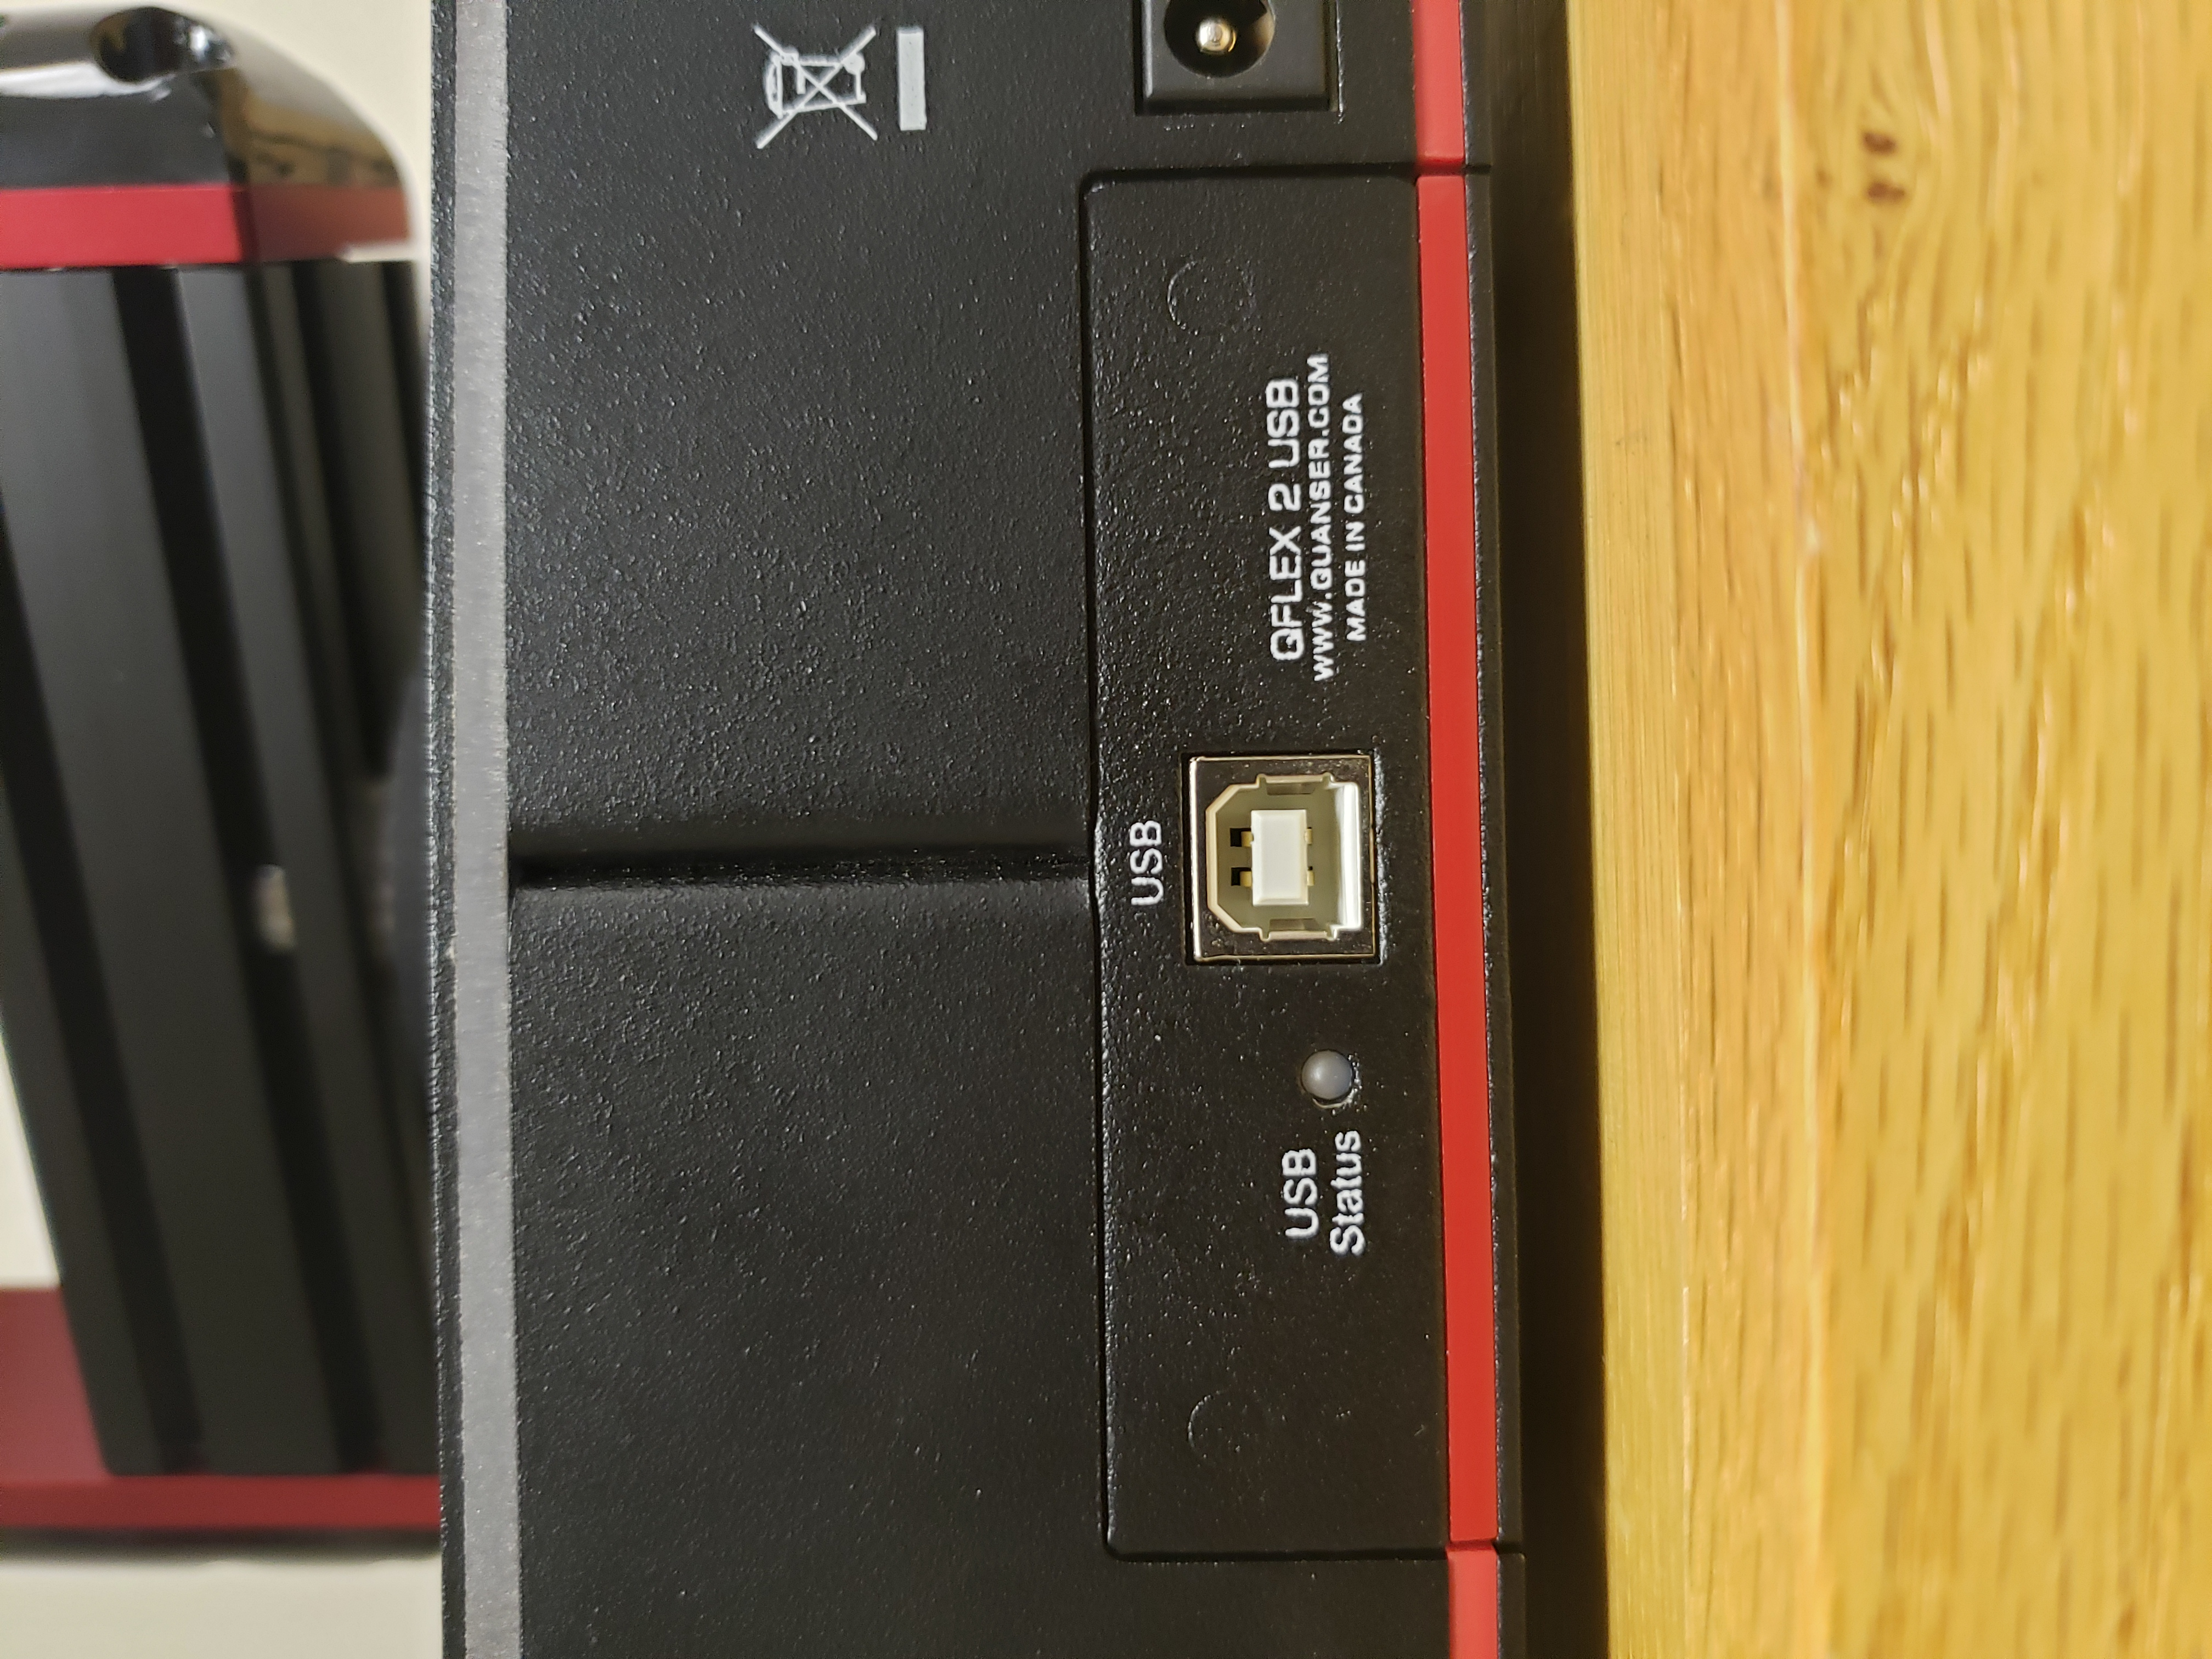
\includegraphics[angle = 270,width=.248\textwidth,keepaspectratio=true]{figs/img/USB_Panel.jpg}
    \label{fig:USB_Panel}
    \caption{Quanser Aero with QFLEX 2 USB panel installed}
\end{figure}
%----------------------------------------------------------------------
\section{Raspberry Pi Implementation}
\label{sec:RPItut}
%----------------------------------------------------------------------
\begin{enumerate}
    \item Make sure software add ons are installed on MATLAB
    \begin{enumerate}
        \item MATLAB Support Package for Raspberry Pi Hardware
        \item Simulink Support Package for Raspberry Pi Hardware
    \end{enumerate}
    \item Install QFLEX 2 EMBEDDED into Quanser Aero as seen in figure~\ref{fig:Embedded_Panel}
    \item Assuming Raspberry PI is not connected to network, establish a serial connection to the Raspberry PI
    \begin{enumerate}
	\item Plug SD card into Linux computer and enable serial connectivity
   	\item Insert SD card back into Raspberry Pi
	\item Connect serial cable to the Raspberry Pi, Pin 3 (black wire), Pin 4 (white wire), Pin 5 (green wire)
	\item Plug Raspberry Pi into commputer
	\item Locate COM port for the connection
	\item Open Putty, select Serial connection, input COM number and 115200 as the speed
	\item Log into Raspberry Pi
	\item Configure network, type "sudo nano /etc/wpa\_supplicant/wpa\_supplicant.conf" and add network settings
    \end{enumerate}
    \item Connect SPI wires to Raspberry PI. Pin 1 (white wire) on the embedded panel connects to +5V on the Pi.  Pin 2 (yellow wire) connects to GPIO 10 on the Pi. Pin 3 (blue wire) connects to GPIO 9 on the Pi.  Pin 4 (green wire) connects to GPIO 11 on the Pi. Pin 6 (purple wire) connects to GPIO 8 on the Pi.  Pin 7 (Red wire) connects to ground on the Pi.
    \item Connect Raspberry PI to QFLEX 2 Embedded
    \item Right click on Simulink model
    \item Open "Model Configuration Parameters"
    \item Select "Hardware Implementation"
    \item Set "Hardware Board" to "Raspberry Pi"
    \item Under "Board Parameters" under "Groups" type in the IP address of the Raspberry PI, the username, and password
    \item Under "Build options", set build action to "Build and run" and type in the file path that you want the model to be stored on the Raspberry PI
    \item Set simulation mode to external
    \item Run MATLAB initialization code for motion controller
    \item Run MATLAB Raspberry PI/SPI initialization code in section~\ref{ch:RPI3_SPI_Int}
    \item Click "Deploy to Hardware" button
    \item To stop program you must "kill" it
    \item Open Putty, connect to your Raspberry PI, and log in
    \item Type "ps -A" to view running programs and find the process number of your Simulink model
    \item Type "sudo kill -9 \#\#\#\#" where \#\#\#\# is your process number.  This will kill the program
    \item To run a file already on the Raspberry Pi use the command "sudo FILEPATH/FILENAME.elf", if file is in current directory use "sudo ./FILENAME.elf"
    \item If the model runs to time infinity when started from the Raspberry Pi you can use Control-C to stop the model
\end{enumerate}

\begin{figure}[!h]
    \centering
    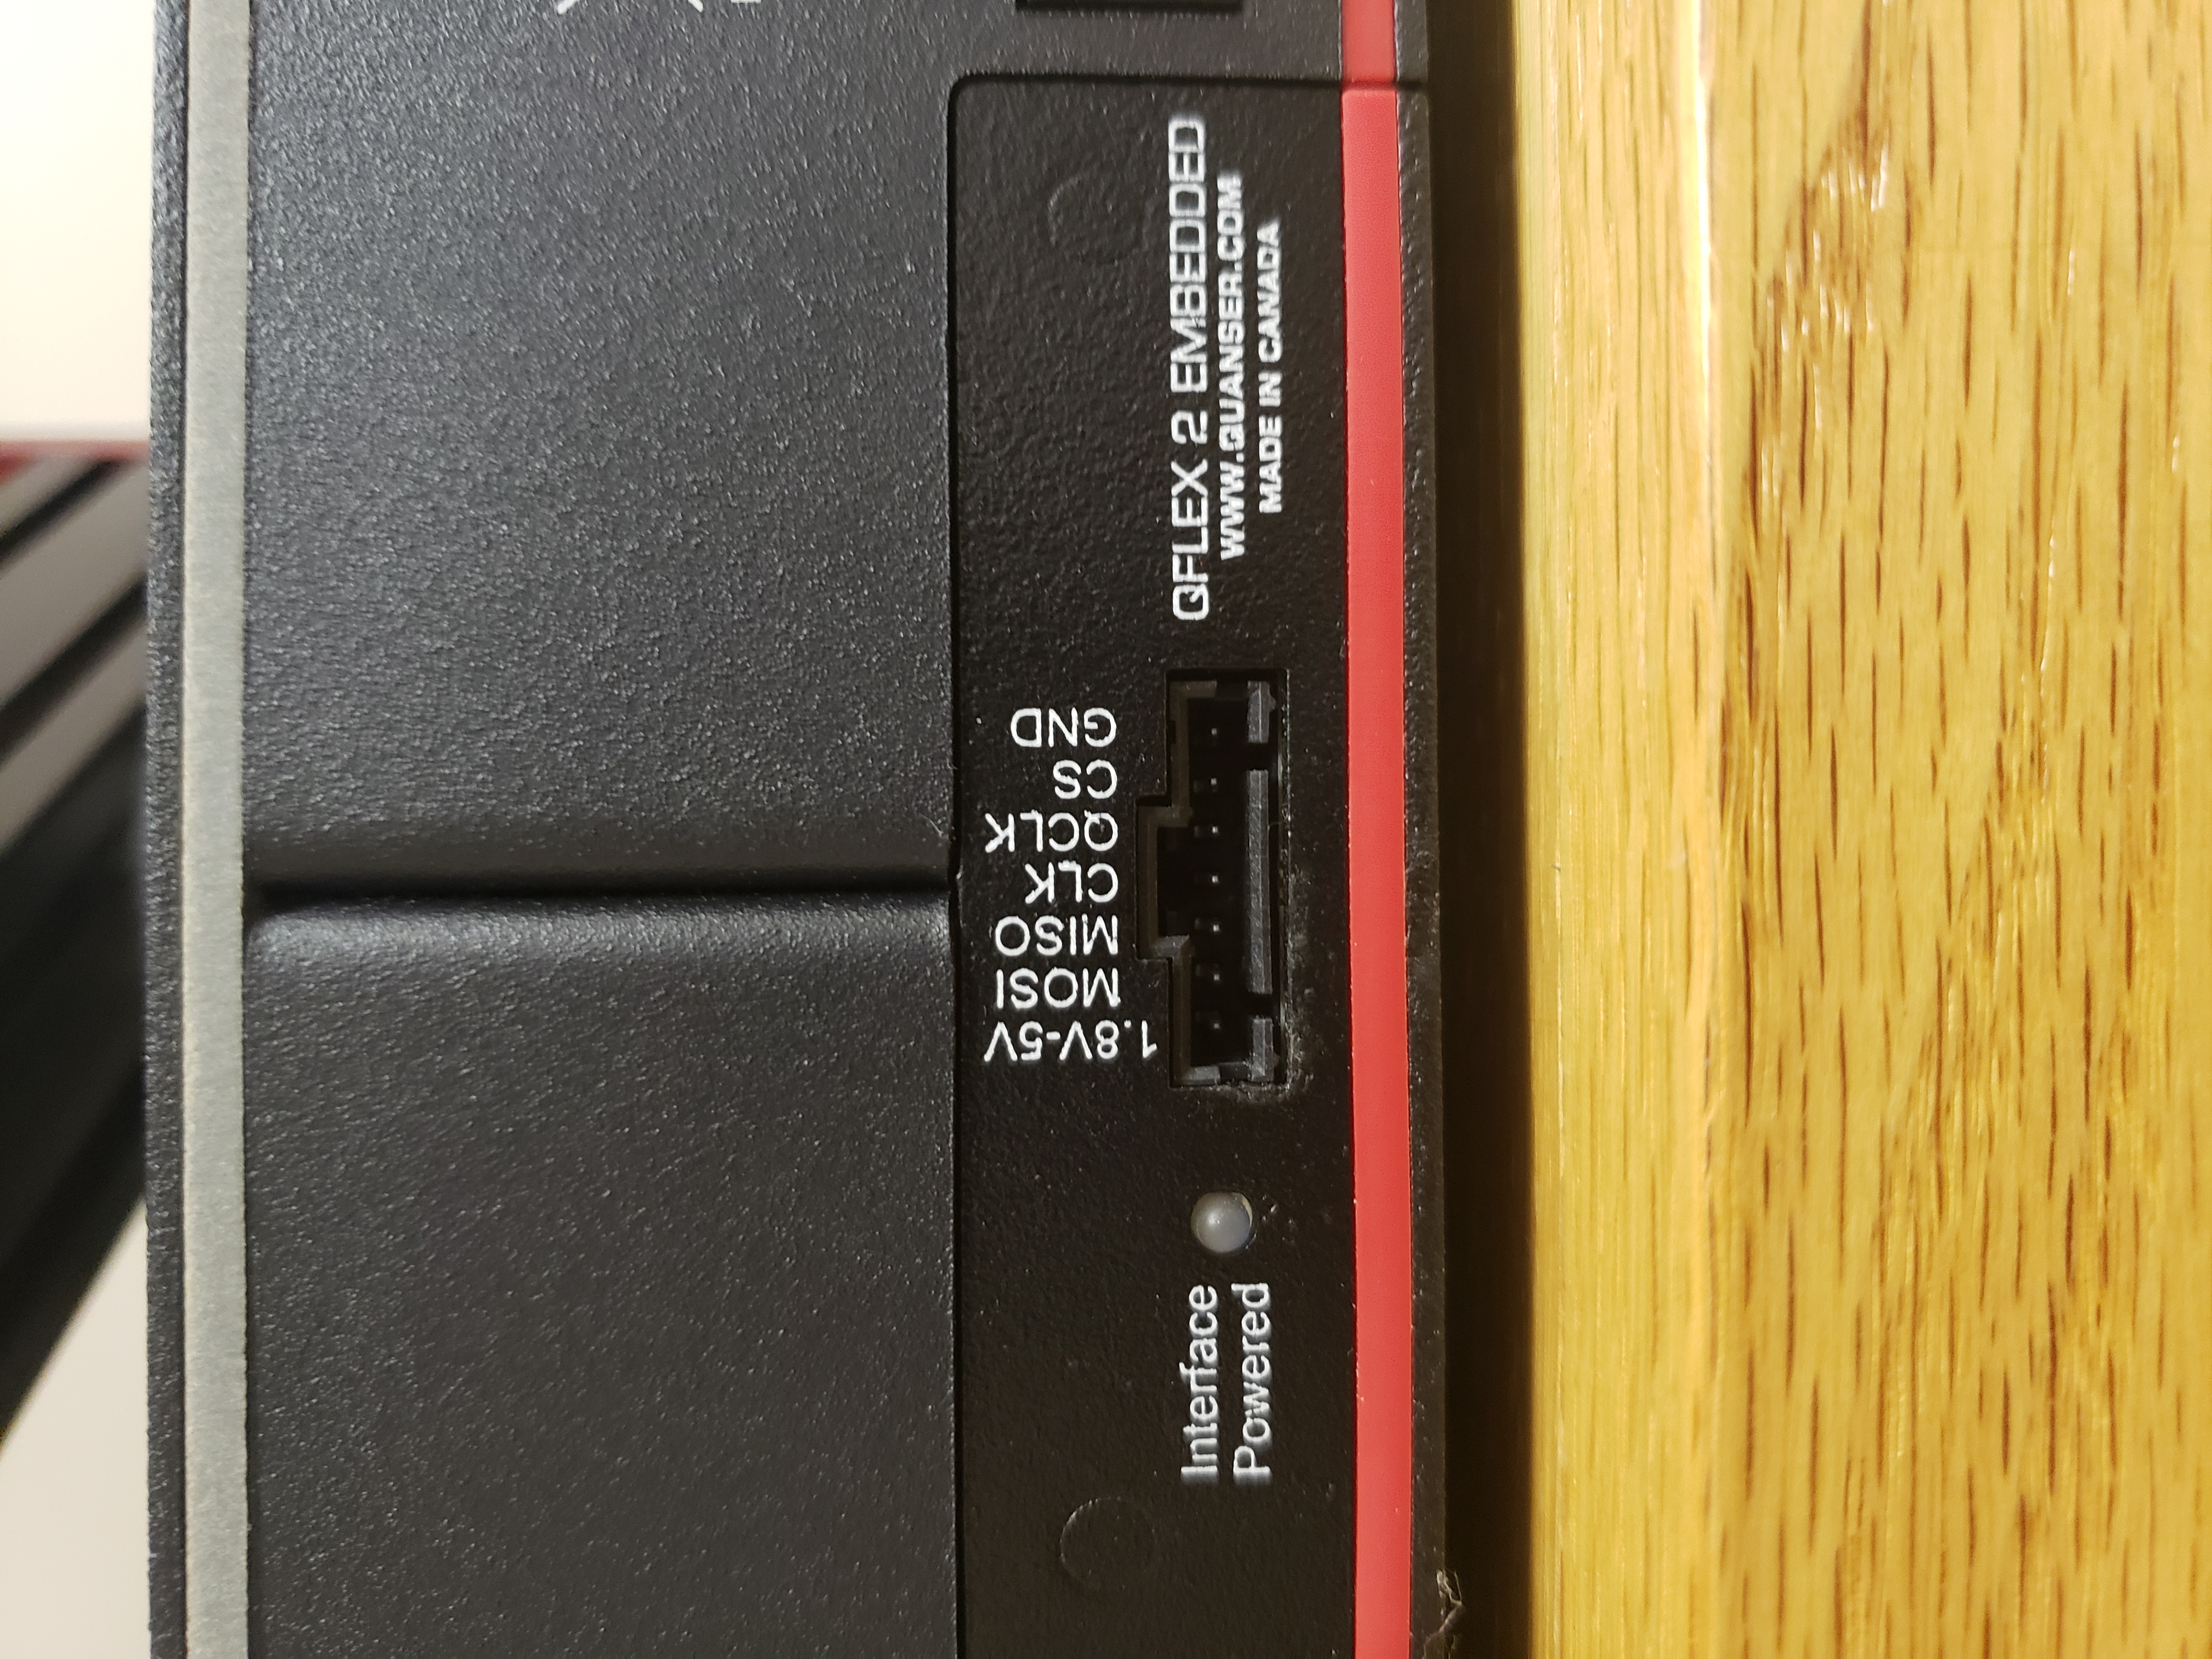
\includegraphics[angle = 270,width=.248\textwidth,keepaspectratio=true]{figs/img/Embedded_Panel.jpg}
    \label{fig:Embedded_Panel}
    \caption{Quanser Aero with QFLEX 2 Embedded panel installed}
\end{figure}
%----------------------------------------------------------------------
\section{Android Application}
\label{sec:Androidtut}
%----------------------------------------------------------------------
\begin{enumerate}
    \item Make sure software add ons are installed on MATLAB, "Simulink Support Package for Android Devices"
    \item Install Android Studio
    \item Repeat steps from appendix~\ref{sec:RPItut} to set up Raspberry Pi and push model to Raspberry Pi
    \item From MATLAB open add on manager and click on the "Setup" gear next to the Android package
    \item Verify Android Studio installed, Next
    \item Verify Android SDK Tools installed
    \item NOTE: The recent version of Android Studio removed one of their files that MATLAB needs to build android applications.  Fixed by downloading and installing an older verison of Android Studio NDK bundle (December 2017) and copying over the missing folder into the file path that MATLAB was calling.  This issue might be fixed in a newer version of Android Studio. 
    \item Click next
    \item Follow intrustions on prompts to turn android on in developer mode
    \item Turn on USB debugging
    \item Install driver
    \item Connect android to computer with USB cable
    \item Allow USB debugging
    \item Make sure both computer and android are on same network with internet access
    \item Select device
    \item Build and run Test App, App should close and delete itself after test is complete
    \item Open simulink model's configuration parameters
    \item Under "Hardware Implementation" set "Hardware Board" to "Android Device"
    \item Build and deploy simulink model to android
    \item Once APP is running, swtich network to same network as the Raspberry Pi
    \item Execute code on Raspberry Pi
    \item Control helicopter
\end{enumerate}

%%% Local Variables:
%%% mode: latex
%%% TeX-master: "../finalReport"
%%% End:
